\documentclass[12pt,tikz]{standalone}
\pdfinfoomitdate 1
\pdfsuppressptexinfo 1
\pdftrailerid{}
\usepackage[utf8]{inputenc}
\usepackage{amsmath}
\usepackage{pgfplots}
\usepackage{tikz}
\pagestyle{empty}

\begin{document}
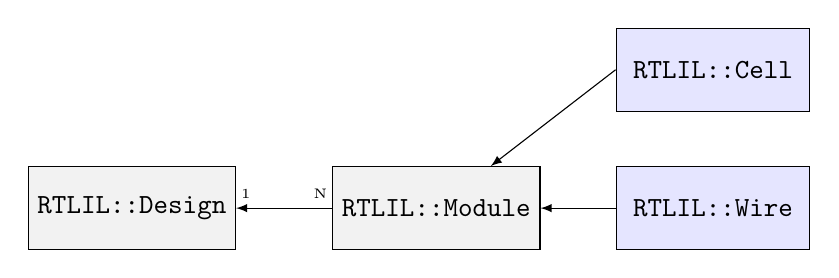
\begin{tikzpicture}[every node/.style={transform shape}]
	\tikzstyle{entity} = [draw, fill=gray!10, rectangle, minimum height=3em, minimum width=7em, node distance=5em, font={\ttfamily}]
	\node[entity] (design) {RTLIL::Design};
	\node[entity] (module) [right of=design, node distance=11em] {RTLIL::Module} edge [-latex] node[above] {\tiny 1 \hskip3em N} (design);

	\node[entity] (wire) [fill=blue!10, right of=module, node distance=10em] {RTLIL::Wire} (wire.west) edge [-latex] (module);
	\node[entity] (cell) [fill=blue!10, above of=wire] {RTLIL::Cell} (cell.west) edge [-latex] (module);
\end{tikzpicture}
\end{document}
